Since our training dataset is sourced from the internet, it is possible that our model was trained on some of our benchmark test sets.  Accurately detecting test contamination from internet-scale datasets is a new area of research without established best practices. While it is common practice to train large models without investigating contamination, given the increasing scale of pretraining datasets, we believe this issue is becoming increasingly important to attend to.

This concern is not just hypothetical. One of the first papers to train a language model on Common Crawl data \cite{trinh2018simple} detected and removed a training document which overlapped with one of their evaluation datasets. Other work such as GPT-2 \cite{radford2019language} also conducted post-hoc overlap analysis. Their study was relatively encouraging, finding that although models did perform moderately better on data that overlapped between training and testing, this did not significantly impact reported results due to the small fraction of data which was contaminated (often only a few percent).

GPT-3 operates in a somewhat different regime.  On the one hand, the dataset and model size are about two orders of magnitude larger than those used for GPT-2, and include a large amount of Common Crawl, creating increased potential for contamination and memorization.  On the other hand, precisely due to the large amount of data, even GPT-3 175B does not overfit its training set by a significant amount, measured relative to a held-out validation set with which it was deduplicated (Figure \ref{graph:training_curves}).  Thus, we expect that contamination is likely to be frequent, but that its effects may not be as large as feared.

We initially tried to address the issue of contamination by proactively searching for and attempting to remove any overlap between our training data and the development and test sets of all benchmarks studied in this paper. Unfortunately, a bug resulted in only partial removal of all detected overlaps from the training data. Due to the cost of training, it wasn't feasible to retrain the model. To address this, we investigate in detail how the remaining detected overlap impacts results.

For each benchmark, we produce a `clean' version which removes all potentially leaked examples, defined roughly as examples that have a 13-gram overlap with anything in the pretraining set (or that overlap with the whole example when it is shorter than 13-grams). The goal is to very conservatively flag anything that could potentially be contamination, so as to produce a clean subset that is free of contamination with high confidence. The exact procedure is detailed in Appendix \ref{appendix:test_set_contamination}.

We then evaluate GPT-3 on these clean benchmarks, and compare to the original score.  If the score on the clean subset is similar to the score on the entire dataset, this suggests that contamination, even if present, does not have a significant effect on reported results.  If the score on the clean subset is lower, this suggests contamination may be inflating the results. The results are summarized in Figure \ref{graph:contamination}.  Although potential contamination is often high (with a quarter of benchmarks scoring over 50\%), in most cases performance changes only negligibly, and we see no evidence that contamination level and performance difference are correlated.  We conclude that either our conservative method substantially overestimated contamination or that contamination has little effect on performance.

Below, we review in more detail the few specific cases where either (1) the model performs significantly worse on the cleaned version, or (2) potential contamination is very high, which makes measuring the performance difference difficult.

\begin{figure}
\centering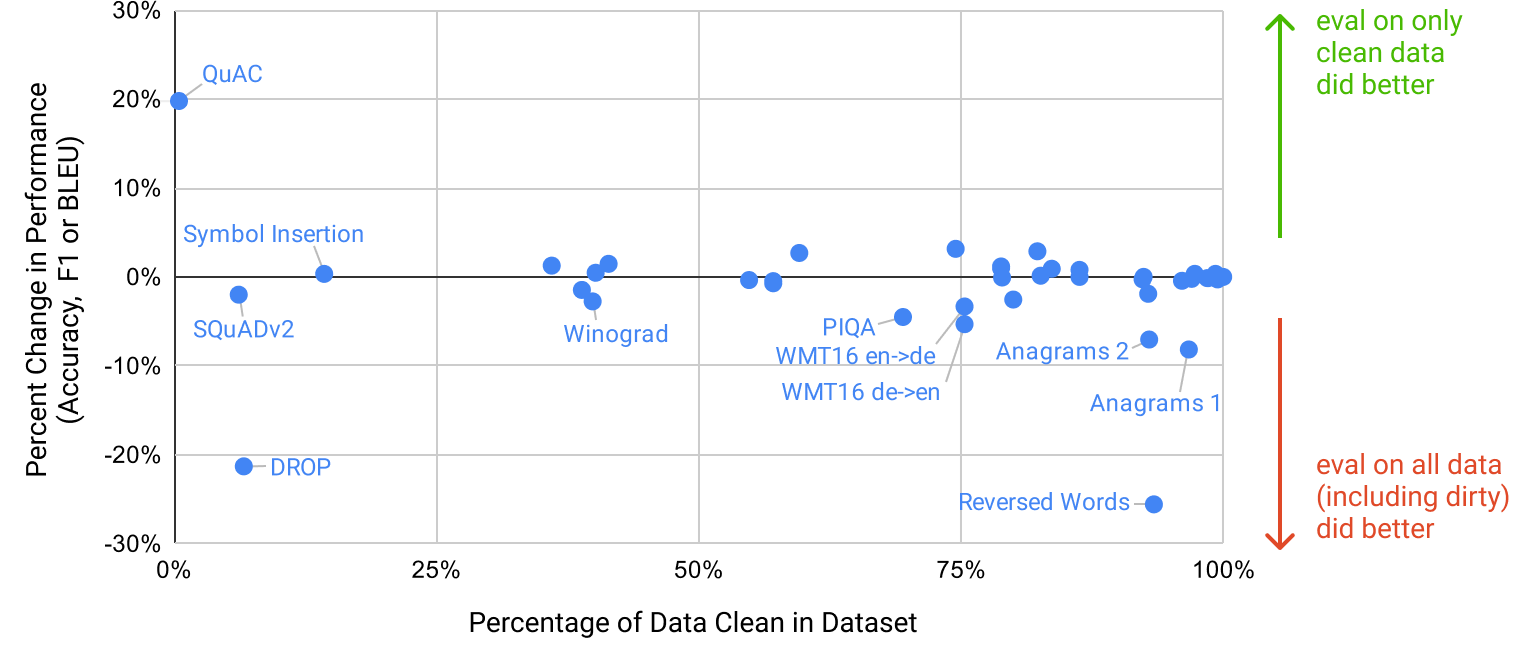
\includegraphics[width=0.9\linewidth]{figures/contamination_graph.png}

\caption{\textbf{Benchmark contamination analysis}~~~ We constructed cleaned versions of each of our benchmarks to check for potential contamination in our training set. The x-axis is a conservative lower bound for how much of the dataset is known with high confidence to be clean, and the y-axis shows the difference in performance when evaluating only on the verified clean subset.  Performance on most benchmarks changed negligibly, but some were flagged for further review.  On inspection we find some evidence for contamination of the PIQA and Winograd results, and we mark the corresponding results in Section \ref{section:Results} with an asterisk. We find no evidence that other benchmarks are affected.}
\label{graph:contamination}
\end{figure}

Our analysis flagged six groups of benchmarks for further investigation: Word Scrambling, Reading Comprehension (QuAC, SQuAD2, DROP), PIQA, Winograd, language modeling tasks (Wikitext tasks, 1BW), and German to English translation. Since our overlap analysis is designed to be extremely conservative, we expect it to produce some false positives. We summarize the results for each group of tasks below:
\begin{itemize}
    \item \textbf{Reading Comprehension:} Our initial analysis flagged $>$90\% of task examples from QuAC, SQuAD2, and DROP as potentially contaminated, so large that even measuring the differential on a clean subset was difficult. Upon manual inspection, however, we found that for every overlap we inspected, in all 3 datasets, the source text was present in our training data but the question/answer pairs were not, meaning the model gains only background information and cannot memorize the answer to a specific question.
    \item \textbf{German translation:} We found 25\% of the examples in the WMT16 German-English test set were marked as potentially contaminated, with an associated total effect size of 1-2 BLEU.  Upon inspection, none of the flagged examples contain paired sentences resembling NMT training data and collisions were monolingual matches mostly of snippets of events discussed in the news.
    \item \textbf{Reversed Words and Anagrams:} Recall that these tasks are of the form ``\texttt{alaok = koala}". Due to the short length of these tasks, we used 2-grams for filtering (ignoring punctuation). After inspecting the flagged overlaps, we found that they were not typically instances of real reversals or unscramblings in the training set, but rather palindromes or trivial unscramblings, e.g ``\texttt{kayak = kayak}". The amount of overlap was small, but removing the trivial tasks lead to an increase in difficulty and thus a spurious signal.  Related to this, the symbol insertion task shows high overlap but no effect on performance -- this is because that task involves removing non-letter characters from a word, and the overlap analysis itself ignores such characters, leading to many spurious matches.
    \item \textbf{PIQA:} The overlap analysis flagged 29\% of examples as contaminated, and observed a 3 percentage point absolute decrease (4\% relative decrease) in performance on the clean subset. Though the test dataset was released after our training set was created and its labels are hidden, some of the web pages used by the crowdsourced dataset creators are contained in our training set. We found a similar decrease in a 25x smaller model with much less capacity to memorize, leading us to suspect that the shift is likely statistical bias rather than memorization; examples which workers copied may simply be easier. Unfortunately, we cannot rigorously prove this hypothesis.  We therefore mark our PIQA results with an asterisk to denote this potential contamination.
    \item \textbf{Winograd:} The overlap analysis flagged 45\% of examples, and found a 2.6\% decrease in performance on the clean subset. Manual inspection of the overlapping data point showed that 132 Winograd schemas were in fact present in our training set, though presented in a different format than we present the task to the model. Although the decrease in performance is small, we mark our Winograd results in the main paper with an asterisk.
    \item \textbf{Language modeling:} We found the 4 Wikipedia language modeling benchmarks measured in GPT-2, plus the Children's Book Test dataset, to be almost entirely contained in our training data.  Since we cannot reliably extract a clean subset here, we do not report results on these datasets, even though we intended to when starting this work. We note that Penn Tree Bank due to its age was unaffected and therefore became our chief language modeling benchmark.
\end{itemize}

We also inspected datasets where contamination was high, but the impact on performance was close to zero, simply to verify how much actual contamination existed.  These appeared to often contain false positives. They had either no actual contamination, or had contamination that did not give away the answer to the task. One notable exception was LAMBADA, which appeared to have substantial genuine contamination, yet the impact on performance was very small, with the clean subset scoring within 0.5\% of the full dataset.  Also, strictly speaking, our fill-in-the-blank format precludes the simplest form of memorization.  Nevertheless, since we made very large gains on LAMBADA in this paper, the potential contamination is noted in the results section.

An important limitation of our contamination analysis is that we cannot be sure that the clean subset is drawn from the same distribution as the original dataset.  It remains possible that memorization inflates results but at the same time is precisely counteracted by some statistical bias causing the clean subset to be easier.  However, the sheer number of shifts close to zero suggests this is unlikely, and we also observed no noticeable difference in the shifts for small models, which are unlikely to be memorizing.

Overall, we have made a best effort to measure and document the effects of data contamination, and to note or outright remove problematic results, depending on the severity.  Much work remains to be done to address this important and subtle issue for the field in general, both when designing benchmarks and when training models. For a more detailed explanation of our analysis, we refer the reader to Appendix \ref{appendix:test_set_contamination}.
